\chapter{数据库设计}
\section{数据库环境说明}
%本系统的数据系统采用MySQL/PostgreSQL/Microsoft SQL Server数据库系统。

%其中xxx模块因为xxx而需要用到Hadoop架构。

本系统的数据系统采用MySQL数据库系统。

\section{数据库的命名规则}
是否允许单词缩写,允许的单词缩写有哪些。
%允许单词缩写
%identity - ID
%password - pw

表名是单数还是复数。关联表如何命名。字符数限制等。

字段是否带上前缀(如integer类型则加上i前缀等)。
%不带

\section{逻辑设计}
%是否需要满足某一种范式。
逻辑设计需要满足BCNF范式。
\begin{figure}[h]
	\centering
	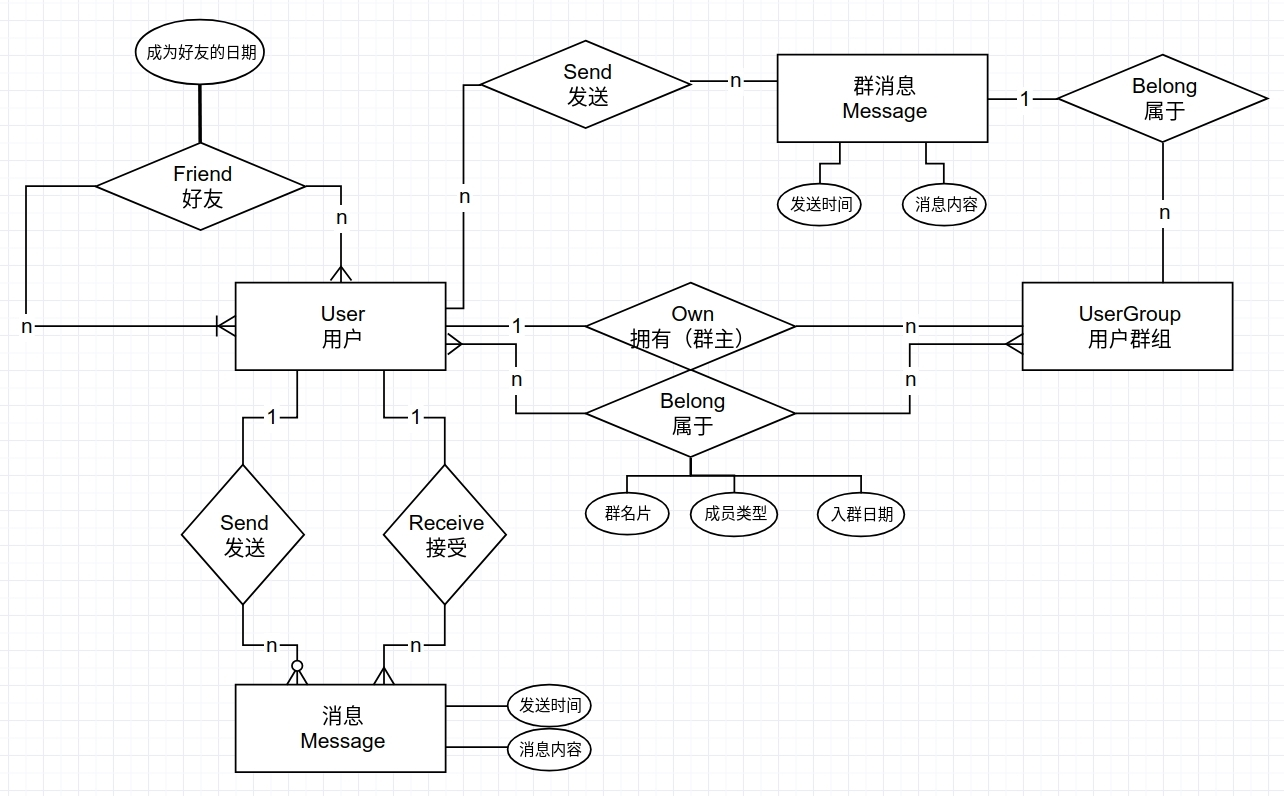
\includegraphics[width=15cm]{er_graph.jpg}
	\caption{用户搜索界面} \label{fig:er_graph}
\end{figure}
服务端数据库的E-R图如图-\ref{fig:er_graph}:。

\section{物理设计}
\subsection{数据库产品}
%用哪家数据库,是否分布式等。
使用MySQL 8.0。由于本产品可自主搭建与部署,且设计为小规模用户使用,故未考虑分布式存储需求。

\subsection{实体属性、类型、精度}
\subsubsection{客户数据表设计}

\begin{table}[htbp]
	\centering
	\caption{用户数据表Users设计} \label{tab:client-database}
	\begin{tabular}{|c|c|c|c|c|}
		\hline
		字段名       & 类型 & 大小 & 说明                 & 备注 \\
		\hline
		ID           & char & 64   & 用户的唯一标识符     & 主键 \\
		\hline
		pw           & char & 512  & 用户的登录密码hash值 & ·    \\
		\hline
		email        & char & 64   & 用户的注册邮箱       & 唯一 \\
		\hline
		lastlogin    & DateTime & 16   & 最近登录时间         & ·    \\
		\hline
		registertime & DateTime & 16   & 注册时间             & ·    \\
		\hline
		birthday     & Date & 16   & 生日                 & ·    \\
		\hline
		sex          & char & 4    & 性别                 & ·    \\
		\hline
		intro        & char & 512  & 个人说明             & ·    \\
		\hline
        avatar       & char & 512  & 头像url              & ·    \\
        \hline
        is\_active   & bool & 1    & 是否在线             & ·    \\
        \hline
        enable\_mobile\_notify & bool & 1 & 移动客户端是否启用消息通知 & · \\
        \hline
        enable\_desktop\_notify & bool & 1 & 桌面客户端是否启用消息通知 & · \\
        \hline
        enable\_sounds & bool & 1  & 是否静音             & ·    \\
        \hline
        default\_language & char & 20 & 默认显示语言       & ·    \\

    \end{tabular}
\end{table}
见表-\ref{tab:client-database}。

\subsubsection{好友数据表设计}
\begin{table}[htbp]
	\centering
	\caption{好友数据表Friends设计} \label{tab:friend-database}
	\begin{tabular}{|c|c|c|c|c|}
		\hline
		字段名 & 类型 & 大小 & 说明           & 备注                 \\
		\hline
		user1  & char & 64   & 用户1          & 外键,来自用户数据表 \\
		\hline
		user2  & char & 64   & 用户2          & 外键,来自用户数据表 \\
		\hline
		time   & Date & 16   & 成为好友的日期 & ·                    \\
		\hline
	\end{tabular}
\end{table}
见表-\ref{tab:friend-database}。

\subsubsection{消息数据表设计}
\begin{table}[htbp]
	\centering
	\caption{消息数据表Messages设计} \label{tab:message-database}
	\begin{tabular}{|c|c|c|c|c|}
		\hline
		字段名  & 类型 & 大小 & 说明             & 备注                 \\
		\hline
		ID      & number & 64   & 消息的唯一标识符 & 主键                 \\
		\hline
		time    & Date & 16   & 发送时间         & ·                    \\
		\hline
		content & char & 1000 & 消息内容         & ·                    \\
		\hline
		from    & char & 64   & 发送者           & 外键,来自用户数据表 \\
		\hline
		to      & char & 64   & 接收者           & 外键,来自用户数据表 \\
		\hline
	\end{tabular}
\end{table}
见表-\ref{tab:message-database}。

\subsubsection{群组消息数据表设计}
\begin{table}[htbp]
	\centering
	\caption{群组消息数据表Messages设计} \label{tab:groupmessage-database}
	\begin{tabular}{|c|c|c|c|c|}
		\hline
		字段名  & 类型 & 大小 & 说明             & 备注                 \\
		\hline
		ID      & number & 64   & 消息的唯一标识符 & 主键                 \\
		\hline
		time    & Date & 16   & 发送时间         & ·                    \\
		\hline
		content & char & 1000 & 消息内容         & ·                    \\
		\hline
		from    & char & 64   & 发送者           & 外键,来自用户数据表 \\
		\hline
		to      & char & 64   & 群组           & 外键,来自群组数据表 \\
		\hline
	\end{tabular}
\end{table}
见表-\ref{tab:groupmessage-database}。

\subsubsection{群组数据表设计}
\begin{table}[htbp]
	\centering
	\caption{群组数据表Groups设计} \label{tab:group-database}
	\begin{tabular}{|c|c|c|c|c|}
		\hline
		字段名     & 类型 & 大小 & 说明             & 备注                 \\
		\hline
		ID         & number & 64   & 群组的唯一标识符 & 主键                 \\
		\hline
		name       & char & 64   & 群名             & ·                    \\
		\hline
		intro      & char & 512  & 简介             & ·                    \\
		\hline
		createtime & Date & 16   & 创建日期         & ·                    \\
		\hline
		user       & char & 64   & 群主             & 外键,来自用户数据表 \\
		\hline
	\end{tabular}
\end{table}
见表-\ref{tab:group-database}。

\subsubsection{群组成员数据表设计}
\begin{table}[htbp]
	\centering
	\caption{群组成员数据表设计} \label{tab:usergroup-database}
	\begin{tabular}{|c|c|c|c|c|}
		\hline
		字段名     & 类型 & 大小 & 说明     & 备注                 \\
		\hline
		user       & char & 64   & 用户     & 外键,来自用户数据表 \\
		\hline
		group       & number & 64   & 群组     & 外键,来自群组数据表 \\
		\hline
		name       & char & 512  & 群名片   & ·                    \\
		\hline
		type       & char & 4    & 成员类型 & ·                    \\
		\hline
		createtime & Date & 16   & 入群日期 & ·                    \\
		\hline
	\end{tabular}
\end{table}
见表-\ref{tab:usergroup-database}。


\section{安全性设计}
%备份和容灾设计。
本产品的服务端主要面向有自己搭建即时通讯服务需求的个人用户和中小企业用户,
预期使用规模较小,所以没有特别的容灾设计,
数据备份工作依靠服务端维护人员自行开展。

\section{数据库管理与维护说明}
对于数据库的维护,随时对数据库中的信息加以调试和保存备份。同样需要个工作人员进行系统的分析和用户的反馈,对系统进行升级以及功能的完善。同时保证系统安全有序的运行。